%% Adaptado de 
%% http://www.ctan.org/tex-archive/macros/latex/contrib/IEEEtran/
%% Traduzido para o congresso de IC da USP
%%*****************************************************************************
% Não modificar

\documentclass[twoside,conference,a4paper]{IEEEtran}

%******************************************************************************
% Não modificar
\usepackage{IEEEtsup} % Definições complementares e modificações.
\usepackage[utf8]{inputenc} % Disponibiliza acentos.
\usepackage[english,brazil]{babel}
%% Disponibiliza Inglês e Português do Brasil.
\usepackage{latexsym,amsfonts,amssymb} % Disponibiliza fontes adicionais.
\usepackage{theorem} 
\usepackage[cmex10]{amsmath} % Pacote matemático básico 
\usepackage{url} 
%\usepackage[portuges,brazil,english]{babel}
\usepackage{graphicx}
\usepackage{amsmath}
\usepackage{amssymb}
\usepackage{color}
\usepackage[pagebackref=true,breaklinks=true,letterpaper=true,colorlinks,bookmarks=false]{hyperref}
\usepackage[tight,footnotesize]{subfigure} 
\usepackage[noadjust]{cite} % Disponibiliza melhorias em citações.
%%*****************************************************************************

\begin{document}
\selectlanguage{brazil}
\renewcommand{\IEEEkeywordsname}{Palavras-chave}

%%*****************************************************************************

\urlstyle{tt}
% Indicar o nome do autor e o curso/nível (grad-mestrado-doutorado-especial)
\title{P2 - Simulador Robótico}
\author{%
 \IEEEauthorblockN{Isadora Sophia Garcia Rodopoulos\,\IEEEauthorrefmark{1}\\
                   Renato Landim Vargas\,\IEEEauthorrefmark{1}}
 \IEEEauthorblockA{\IEEEauthorrefmark{1}%
                   Ciência da Computação - Graduação - RA 158018\\
                   E-mail: ra158018@ic.unicamp.br}
 \IEEEauthorblockA{\IEEEauthorrefmark{1}%
                   Ciência da Computação - Graduação - RA 118557\\
                   E-mail: ra118557@ic.unicamp.br}
}

%%*****************************************************************************

\maketitle

%%*****************************************************************************
% Resumo do trabalho
\begin{abstract}
O trabalho se baseou em implementar assuntos teóricos desenvolvidos em sala de aula,
entre eles: explorar métodos de controle mais avançados e computar a odometria
do robô através de um modelo cinemático. Os assuntos são desenvolvidos a partir de
um ambiente com o robô p3dx, com o suporte do \textit{V-REP}.

O objetivo se trata de fazer o robô explorar o cenário e coletar informações relevantes
tanto sobre o ambiente quanto sua localização. A solução foi proposta através
do mapeamento de informações com o Ground Trouth, com o auxílio de gráficos, e utilizando
o modelo cinemático com a odometria para o controle do robô. Para tornar o controle
mais robusto, foi utilizado métodos como o sistema \textbf{fuzzy}, para que o robô
possa acompanhar as paredes, desviar de obstáculos e evitar ficar preso.

O resultado (???) to continue
% O resumo deve conter uma breve descrição sobre várias partes do seu trabalho que serão tratadas no decorrer do texto. Primeiramente, pode-se descrever brevemente o problema no qual você está trabalhando: Por que você está desenvolvendo este trabalho? Qual a motivação para este desenvolvimento? Por que ele é importante? O resumo deve conter também um breve descritivo da metodologia que você usou no desenvolvimento: Que problema foi tratado? Como a solução foi construída/desenvolvida? Quais as tecnologias utilizadas? Finalmente, deve falar um pouco sobre os resultados que você conseguiu: o resultado final ficou bom? Quais os seus principais diferenciais? Qual a eficiência do desenvolvimento?
\end{abstract}

% Indique três palavras-chave que descrevem o trabalho
\begin{IEEEkeywords}
fuzzy, odometria, sistemas inteligentes.
\end{IEEEkeywords}

%%*****************************************************************************
% Modifique as seções de acordo com o seu projeto

\section{Introdução}
O projeto foi baseado na literatura proposta em sala de aula e 

Na introdução você deve descrever os aspectos mais relevantes sobre a revisão bibliográfica que fez e do problema que você decidiu tratar. Quais foram os pontos estudados/pesquisados? Quais os outros trabalhos similares ao seu que você encontrou? 

Também na introdução espera-se que você descreva um pouco sobre a motivação de trabalhar com esse tema. A descrição do seu trabalho será feita em detalhes nas próximas seções do artigo.

No final da introdução, é comum inserir um parágrafo descrevendo o que será encontrado em cada seção no restante do seu texto. Exemplo: Este trabalho encontra-se organizado da seguinte forma: a seção 2 apresenta X. A seção 3 descreve Y. Os resultados são apresentados na seção 4, e as conclusões são apresentadas na seção 5.

\section{Seções}

Utilize outras seções e subseções para abordar o problema. 

\subsection{Uma subseção}

Se precisar, você pode usar listas, tais como

\begin{itemize}
 \item Item 1
 \item Item 2
\end{itemize}
ou
\begin{enumerate}
 \item Item 1
 \item Item 2
\end{enumerate}

\section{Trabalho Proposto}

Nesta seção descreva de forma abrangente, porém clara e organizada, o seu trabalho.

\subsection{Tabelas}

Uma tabela pode ser posicionada em qualquer lugar no texto, como no exemplo
seguinte.
%
\begin{table}[ht]
\renewcommand{\arraystretch}{1.3}
\centering
 \caption{Exemplo de texto de uma tabela.}
 \label{tab:tab1}
 \begin{tabular}{lcccc}\hline
  & \multicolumn{2}{c}{Texto}
  & \multicolumn{2}{c}{Sem \#21} \\ \cline{2-5}
  X & Y & $z$ & $\mathcal{A}$ & valor-$z$ \\ \hline \hline
  1      &0,491  & 3,66   &0,367 &2,46  \\
  2    &0,732  & 4,21   &0,354 &1,50  \\
  3      &0,000  & -      &0,000 & -    \\
  4      &0,000  & -      &0,000 & -  \\
  5      &0,421  & 1,94   &0,668 &2,79  \\
  6      &0,421  & 1,94   &0,668 &2,79  \\
  7      &0,938  & 3,92   &1,295 &4,67 \\
  8       &0,000  & -      &0,000 & - \\
  9       &0,356  & 1,40   &0,491 &1,87 \\ \hline
 \end{tabular}
\end{table}

Para citar esta tabela, em qualquer ponto no texto, como Tabela~\ref{tab:tab1}.


\section{Materiais e Métodos}

Todo trabalho deve ser submetido a algum tipo de teste para que possa ser avaliado. Na verdade, buscamos aqui uma validação com um caráter mais científico de seu trabalho (validação de hipótese). Busca-se identificar quais os seus pontos fortes e fracos. Nesta seção você deve descrever claramente quais foram e como foram conduzidos os testes, quais os materiais e as metodologias empregadas.   

Uma figura pode ser posicionada em qualquer lugar no texto, como no exemplo seguinte da Figura~\ref{fig:fig1}.

\begin{figure}[ht]
\centering
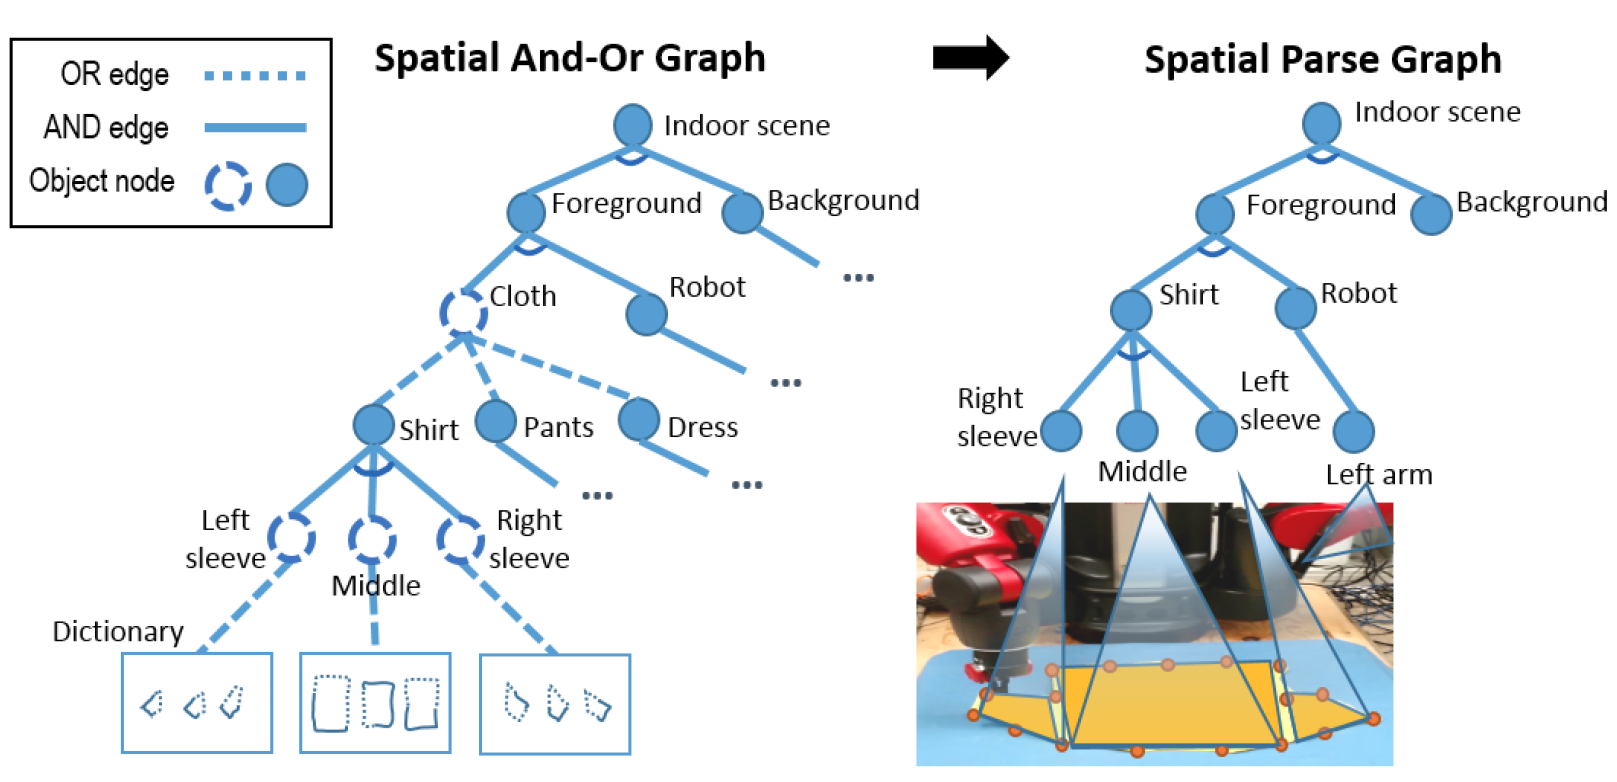
\includegraphics[width=1\hsize]{figuras/pipeline.png}
\caption{Um exemplo de figura.}
\label{fig:fig1}
\end{figure}

Use o comando ``cite'' para citar itens na sua lista de
referências através dos seus rótulos. Exemplo: \cite{Rowling:1997}\cite{Reynolds:2009a}\cite{Michalowski:2006}.


\section{Resultados e Discussão}

Nesta seção você deve apresentar claramente os resultados obtidos para os testes efetuados. Procure organizar os dados utilizando uma linguagem científica. Algumas opções são o uso de tabelas e gráficos, para que a compreensão seja fácil e rápida. 

\section{Conclusões}

Nesta seção, faça uma análise geral de seu trabalho, levando em conta todo o processo de desenvolvimento e os resultados. Quais os seus pontos fortes? Quais os seus pontos fracos? Quais aspectos de sua metodologia de trabalho foram positivas? Quais foram negativas? O que você recomendaria (ou não recomendaria) a outras pessoas que estejam realizando trabalhos similares aos seus? 


%******************************************************************************
% Referências - Definidas no arquivo Relatorio.bib
 +-------------+

\bibliographystyle{IEEEtran}

\bibliography{Relatorio}


%******************************************************************************

\vspace{20ex}

\section*{\Large \textbf{Submissão}}

Seu trabalho deve ser submetido via moodle em conjunto com o código fonte.

\vspace{3ex}


\end{document}
